\begin{figure}[h!]
\centering
\begin{subfigure}[b]{0.25\textwidth}
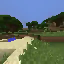
\includegraphics[width=\textwidth]{figures/inputs/image64}
\caption{Dreamer 3 (64$\times$64)}
\end{subfigure}\hfill%
\begin{subfigure}[b]{0.25\textwidth}
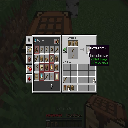
\includegraphics[width=\textwidth]{figures/inputs/image128}
\caption{VPT (128$\times$128)}
\end{subfigure}\hfill%
\begin{subfigure}[b]{0.445\textwidth}
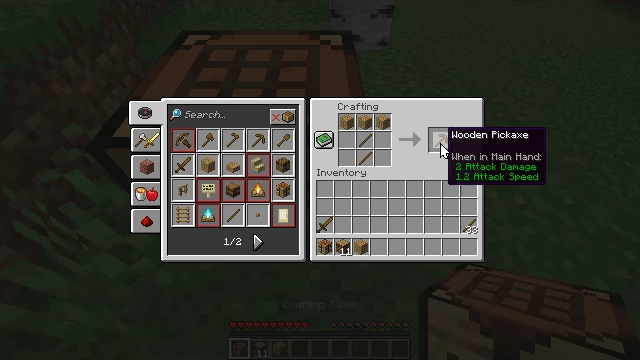
\includegraphics[width=\textwidth]{figures/inputs/image640}
\caption{\method (360$\times$640)}
\end{subfigure}%
\caption{%
Comparison of input images for different agents.
\method learns directly from high-resolution images reflecting the experience of human players.
}
\label{fig:inputs}
\end{figure}
